%!TEX encoding = UTF-8 Unicode
%!TEX root = ../galgas-book.tex

%--------------------------------------------------------------
\chapter{Project Component}\index{Component!Project}
%-------------------------------------------------------------


\section{Generated Cocoa Application}

When a project component is compiled with a Xcode project target, a \texttt{project\_xcode} directory is created. This directory contains:
\begin{itemize}
\item the Xcode project file;
\item a \texttt{build.command} file ;
\item an \texttt{Info.plist} file ;
\item an \texttt{English.lproj} directory ;
\item an empty \texttt{userResources} directory.
\end{itemize}

The \texttt{Info.plist}, the \texttt{English.lproj} directory and the \texttt{userResources} directory are used by the Cocoa target of the Xcode project. The \texttt{build.command} file is a command file that builds the Xcode project.

All files you put in the \texttt{userResources} directory are added to the Cocoa target of the Xcode project when the GALGAS Project component is compiled. When the Cocoa target of the Xcode project is compiled, theses files are put in the \texttt{Resources} directory within the application bundle.

Adding files to the \texttt{userResources} directory is the way of customizing the Cocoa Application:
\begin{itemize}
\item adding icons to your Application (\refSubsectionPage{addingIconsCocoaApplication});
\item customizing syntax coloring (\refSubsectionPage{customizingSyntaxColoring}). 
\end{itemize}




\subsectionLabel{Adding Icons to your Cocoa Application}{addingIconsCocoaApplication}

For setting an icon for your Cocoa application and its documents, proceed as following.



\texteEncercle{1} Design icons, for example with names \texttt{myApplicationIcon.icns} and \texttt{myDocumentIcon.icns}.

\texteEncercle{2} Put the icons in the \texttt{userResources} directory.

\texteEncercle{3} Compile the GALGAS project: this updates the Xcode project, adding the icons files to its Cocoa target.

\texteEncercle{4} Under Xcode, edit the \texttt{Info.plist} file for assigning icon to the application and to the document (see \url{http://developer.apple.com/library/mac/#documentation/Cocoa/Conceptual/Documents/Concepts/DocTypePList.html}).



\subsectionLabel{Customizing Syntax Coloring}{customizingSyntaxColoring}

This feature enables to set particular display attributes to a given list of tokens. This list is defined by a plist file located in the \emph{Resources} directory of the application bundle.

\texteEncercle{1} Edit the GALGAS lexique component, and add one (or more) \motCle{style} entries. For example:

\begin{lstlisting}[language=galgas]
lexique my_lexique :
  ...
style mySpecificStyle -> "My Style" ;
  ...
end lexique ;
\end{lstlisting}

This new style's feature can be edited as other styles, by the Preferences setting of your Cocoa application.


\texteEncercle{2} Create a plist file with the \emph{Property List Editor} application. This file should be named with the lexique component name, suffixed by \texttt{-syntax-coloring-adds}: so, for the example, the file name is \texttt{my\_lexique-syntax-coloring-adds.plist}. Put this file in the \emph{userResources} directory: so when the GALGAS project document is compiled, this file is added to the Cocoa Target of the Xcode project. 

\texteEncercle{3} Edit the \texttt{my\_lexique-syntax-coloring-adds.plist} with the  \emph{Property List Editor} application or Xcode. Add one entry for every custom syntax coloring case: the \emph{key} is the terminal spelling, the \emph{value} has the \emph{String} type, and the specific style name. For example, the \refFigure{}{customSyntaxColoringPropertyList} shows the assignment of the terminal which spelling is \texttt{begin} by the \texttt{mySpecificStyle} style.

\begin{figure}[ht]
  \centering
  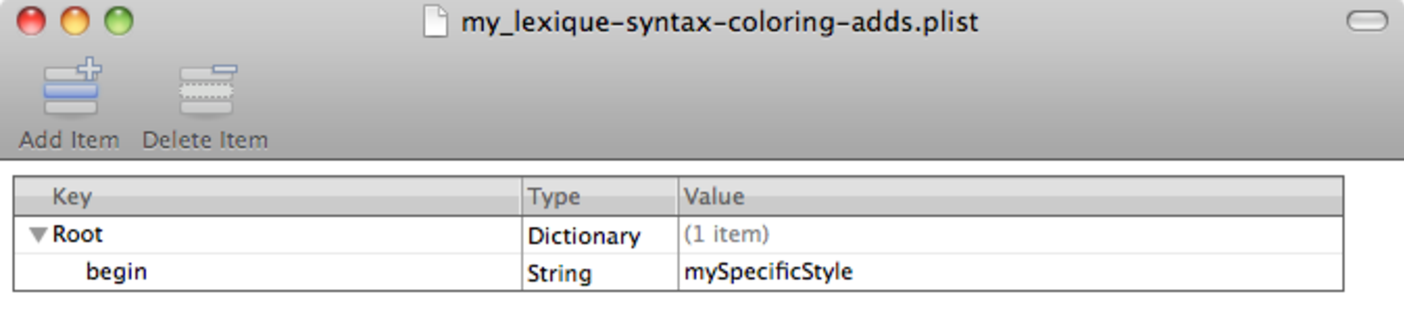
\includegraphics[width=15cm]{chapter-project-component/custom-syntax-coloring-property-list-edition.pdf}
  \caption{Example of a syntax coloring property list}
  \labelFigure{customSyntaxColoringPropertyList}
\end{figure}

If your provides an undefined style name, you will be warned every time you open a document by a beep and a small explanation window.






 
